\documentclass[degree=master, tocarialchapter]{thuthesis}
% 选项
%   degree=[bachelor|master|doctor|postdoctor], % 必选,学位类型
%   secret,                % 可选(默认:关闭),是否有密级
%   tocarialchapter,       % 可选(默认:关闭),章目录中使用黑体(这项表示同时打开下面两项)
%   tocarialchapterentry,  % 可选(默认:关闭),单独控制章标题在目录中使用黑体
%   tocarialchapterpage,   % 可选(默认:关闭),单独控制章页码在目录中使用黑体
%   pifootnote,            % 可选(默认:关闭),页脚编号采用 pifont 字体符号,建议打开

% 所有其它可能用到的包都统一放到这里了,可以根据自己的实际添加或者删除。
\usepackage{thuthesis}
\usepackage{pdfpages}
\usepackage{listings}
\lstset{
	columns=fixed,       
	numbers=left,                                        % 在左侧显示行号
	numberstyle=\tiny\color{gray},                       % 设定行号格式
	frame=none,                                          % 不显示背景边框
	backgroundcolor=\color[RGB]{245,245,244},            % 设定背景颜色
	keywordstyle=\color[RGB]{40,40,255},                 % 设定关键字颜色
	numberstyle=\footnotesize\color{darkgray},           
	commentstyle=\it\color[RGB]{0,96,96},                % 设置代码注释的格式
	stringstyle=\rmfamily\slshape\color[RGB]{128,0,0},   % 设置字符串格式
	showstringspaces=false,                              % 不显示字符串中的空格
	language=matlab,                                        % 设置语言
}

% 定义所有的图片文件在 figures 子目录下
\graphicspath{{figures/}}

% 可以在这里修改配置文件中的定义。导言区可以使用中文。
% \def\myname{薛瑞尼}

\begin{document}


\includepdf{data/cover-converted.pdf}

%%% 封面部分
 \frontmatter
 \thusetup{
  %******************************
  % 注意:
  %   1. 配置里面不要出现空行
  %   2. 不需要的配置信息可以删除
  %******************************
  %
  %=====
  % 秘级
  %=====
  secretlevel={秘密},
  secretyear={10},
  %
  %=========
  % 中文信息
  %=========
  ctitle={误差反向传播神经网络的Matlab实现及应用 \version},
  cdegree={工学硕士},
  cdepartment={计算机科学与技术系},
  cmajor={计算机科学与技术},
  cauthor={杨子棵},
  csupervisor={郑纬民教授},
  cassosupervisor={陈文光教授}, % 副指导老师
  ccosupervisor={某某某教授}, % 联合指导老师
  % 日期自动使用当前时间,若需指定按如下方式修改:
   cdate={超新星纪元},
  %
  % 博士后专有部分
  cfirstdiscipline={计算机科学与技术},
  cseconddiscipline={系统结构},
  postdoctordate={2009年7月——2011年7月},
  id={编号}, % 可以留空: id={},
  udc={UDC}, % 可以留空
  catalognumber={分类号}, % 可以留空
  %
  %=========
  % 英文信息
  %=========
  etitle={An Introduction to \LaTeX{} Thesis Template of Tsinghua University v\version},
  % 这块比较复杂,需要分情况讨论:
  % 1. 学术型硕士
  %    edegree:必须为Master of Arts或Master of Science(注意大小写)
  %             “哲学、文学、历史学、法学、教育学、艺术学门类,公共管理学科
  %              填写Master of Arts,其它填写Master of Science”
  %    emajor:“获得一级学科授权的学科填写一级学科名称,其它填写二级学科名称”
  % 2. 专业型硕士
  %    edegree:“填写专业学位英文名称全称”
  %    emajor:“工程硕士填写工程领域,其它专业学位不填写此项”
  % 3. 学术型博士
  %    edegree:Doctor of Philosophy(注意大小写)
  %    emajor:“获得一级学科授权的学科填写一级学科名称,其它填写二级学科名称”
  % 4. 专业型博士
  %    edegree:“填写专业学位英文名称全称”
  %    emajor:不填写此项
  edegree={Doctor of Engineering},
  emajor={Computer Science and Technology},
  eauthor={Xue Ruini},
  esupervisor={Professor Zheng Weimin},
  eassosupervisor={Chen Wenguang},
  % 日期自动生成,若需指定按如下方式修改:
  % edate={December, 2005}
  %
  % 关键词用“英文逗号”分割
  ckeywords={误差反向传播神经网络, 训练, 测试, Matlab, 分类问题},
  ekeywords={Error Back Propagation Neural Network, Training, Testing, Matlab, Classification problem}
}

% 定义中英文摘要和关键字
\begin{cabstract}
误差反向传播神经网络是一种典型的人工神经网络,在一些数学问题的解决中起到了重要的作用。本文介绍了误差反向传播神经网络的原理和模型,对网络的前向传播和后向传播进行了详细的数学推导,并利用Matlab对网络进行了建模,通过分类问题对所得的模型进行训练、测试、分析,测试结果的正确率均在$99\%$以上,最后对所构建的模型和测试情况进行了简要说明和分析。

本文的创新点主要有:
  \begin{itemize}
  	\item 对误差反向传播神经网络进行了数学推导;
    \item 用Matlab实现误差反向传播神经网络;
    \item 用误差反向传播神经网络解决分类问题。
  \end{itemize}

\end{cabstract}

% 如果习惯关键字跟在摘要文字后面,可以用直接命令来设置,如下:
% \ckeywords{\TeX, \LaTeX, CJK, 模板, 论文}

\begin{eabstract}
  The Error Back Propagation Neural Network is a typical artificial neural network and plays an important role in solving some mathematical problems. This paper introduces the principle and model of the Error Back Propagation Neural Network, and makes a detailed mathematical derivation of the forward and backward propagation of the network, and uses Matlab to model the network, through classification problem. The classification problem is to train, test, and analyze the obtained model. The correct rate of the test results is above $99\%$. Finally, the model and test conditions are briefly described and analyzed.
  
  The main innovations of this paper are:
    \begin{itemize}
  	\item Mathematical Derivation of Error Back Propagation Neural Networks;
  	\item Model Error Back Propagation Neural Network in Matlab;
  	\item Using Error Back Propagation Neural Network to Solve Classification Problems。
  \end{itemize}
\end{eabstract}

% \ekeywords{\TeX, \LaTeX, CJK, template, thesis}

% 如果使用授权说明扫描页,将可选参数中指定为扫描得到的 PDF 文件名,例如:
% \makecover[scan-auth.pdf]
 \makecover

%% 目录
\tableofcontents

%% 符号对照表
\begin{denotation}[3cm]
\item[$Y^{(n)}$]神经网络第$n$层的输入向量 
\item[$Y^{(n)}_{(i)}$]神经网络第$n$层第$i$个神经元的输入
\item[$V^{(n)}$]神经网络第$n$层的输出矩阵
\item[$V^{(n)}_{(i)}$]神经网络第$n$层第$i$个神经元的输出 
\item[$W^{(n)}$]第$n$层与第$n-1$层神经元之间的连接权值矩阵
\item[$W^{(n)}_{ij}$]第$n$层的第$j$个神经元与第$n-1$层的第$i$个神经元之间的连接权值
\item[$\theta^{(n)}$]第$n$层神经元的阈值向量
\item[$\theta^{(n)}_{(i)}$]第$n$层的第$i$个神经元的阈值
\item[$k$]第$n$层神经元的个数
\item[$q$]第$n-1$层神经元的个数
\item[$T$]期望值
\item[$\delta_{i}$]第$i$个神经元与期望值的误差
\item[$\eta$]训练步长
\end{denotation}



%%% 正文部分
\mainmatter
\chapter{误差反向传播神经网络概述}
\label{cha:intro}

在机器学习和认知科学领域中,人工神经网络是一种模仿生物神经网络(动物的中枢神经系统,特别是大脑)的结构和功能的数学模型或计算模型,用于对函数进行估计或近似。神经网络由大量的人工神经元联结进行计算。大多数情况下人工神经网络能在外界信息的基础上改变内部结构,是一种自适应系统。

误差反向传播神经网络\cite{RepresentationsByBP}是一种与最优化方法(如梯度下降法)结合使用的,用来训练人工神经网络的常见方法。该方法对网络中所有权重计算损失函数的梯度。这个梯度会反馈给最优化方法,用来更新权值以最小化损失函数。反向传播要求有对每个输入值想得到的已知输出,来计算损失函数梯度。因此,它通常被认为是一种监督式学习方法,虽然它也用在一些无监督网络中。

误差反向传播神经网络的算法思想是 :让信号正向传播和误差反向传播这两个过程交替循环进行,信号每正向传播一次之后都要计算一次误差,让误差沿梯度负方向下降一个很小的变化量,将这个误差变化量反向传播到神经网络的各层,然后对各层参数矩阵的值进行调整,之后再进行下一次循环。理论上讲,经过多次循环之后,神经网络的误差会收敛到一个较为稳定的范围之内,这时候就可以认为各层参数矩阵的值达到了理想值,即模型达到了最优状态。这种误差反向传播训练算法是人工神经网络的核心思想,当前比较流行的卷积神经网络、循环神经网络等训练算法都是在误差反向传播神经网络算法基础上经过优化和改进发展而来的。\cite{BPNNPrinciple}


\chapter{网络模型与原理}
\label{cha:algorithm}

\section{模型概述}
在神经网络信号的正向传播中,神经元接收到来自其他神经元的输入信号,这些信号乘以权重累加到神经元接收的总输入值上,随后与当前神经元的阈值进行比较,然后通过激活函数处理,产生神经元的输出。理想的激活函数是阶跃函数,然而阶跃函数的缺点是不连续,不可导,所以常用$sigmoid$函数作为误差反向传播神经网络的激活函数。

误差反向传播神经网络的核心思想就是:通过调整各神经元之间的权值,将误差由隐含层向输入层逐层反传,也就是先实现信号的正向传播到误差的反向传播过程。所以误差反向传播神经网络算法的核心步骤如下 :(1)求得在特定输入下实际输出与理想输出的平方误差函数(误差函数或者叫代价函数);(2)利用误差函数对神经网络中的阈值以及连接权值进行求导;(3)根据梯度下降算法,对极小值进行逼近,当满足条件时,跳出循环。

在本篇论文中,将使用的是有监督的误差反向传播神经网络。故我们需要提供一个包括输入和期望输出的训练集,以在训练的过程中获得它相对于训练集的误差。正向传播 :输入样本—输入层—各隐含层—输出层 ;若输出层的实际输出与期望的输出不符,则误差反传 :误差表示—修正各层神经元的权值 ;直到网络输出的误差减少到可以接受的程度,或者进行到预先设定的学习次数为止。

\section{模型推导}

在反向传播神经网络中,通常选择的是$sigmoid$函数作为激活函数,这类函数的导数有一个很好的性质,就是自身相关。$sigmoid$函数如式~(\ref{equ:algorithm:sigmoid})。
\begin{equation}
\label{equ:algorithm:sigmoid}
sigmoid(x) = \frac{1}{1+e^{-x}}
\end{equation}
其导数如式~~(\ref{equ:algorithm:sigmoidDerivative})
\begin{equation}
\label{equ:algorithm:sigmoidDerivative}
sigmoid'(x) = sigmoid(x)(1-sigmoid(x))
\end{equation}
假定现有一个四层的神经网络,包括一层输入层、两层隐含层和一层输出层。假定各层的神经元数量分别为:6,4,3,2。接下来对各层的输入和输出变量进行定义,输入至输入层的输入向量如式~(\ref{equ:algorithm:input0});对应的第一层隐含层的输入向量如式~(\ref{equ:algorithm:input0});第二层隐含层的输入向量为式~(\ref{equ:algorithm:input0});输出层的输入向量为式~(\ref{equ:algorithm:input0})\cite{BPNNPrincipleY}
\begin{equation}
\label{equ:algorithm:input0}
Y^{(0)} = [x_1,x_2,\cdots,x_6]^T =[a_1(0),a_2(0),a_3(0),a_4(0),a_5(0),a_6(0)]^T
\end{equation}
\begin{equation}
\label{equ:algorithm:input1}
Y^{(1)} = [a_1(1),a_2(1),a_3(1),a_4(1)]^T 
\end{equation}
\begin{equation}
\label{equ:algorithm:input2}
Y^{(2)} = [a_1(2),a_2(2),a_3(2)]^T
\end{equation}
\begin{equation}
\label{equ:algorithm:input3}
Y^{(3)} = [a_1(3),a_2(3)]^T
\end{equation}
假定第$n$层($n>=2$)神经元的个数为$i$个,第$n-1$层的神经元个数为$j$个,定义第$n$层与第$n-1$层之间的连接权值矩阵如式~(\ref{equ:algorithm:wMatrix})
\begin{equation}
\label{equ:algorithm:wMatrix}
W^{(n)}=\begin{bmatrix}
w_{11}^{(n)} & \cdots & w_{1j}^{(n)} \\
\vdots & \cdots & \vdots \\
w_{i1}^{(n)}& \cdots & w_{ij}^{(n)}
\end{bmatrix}
\end{equation}
定义第$n$层神经元的阈值向量如式~(\ref{equ:algorithm:thetaVector})
\begin{equation}
\label{equ:algorithm:thetaVector}
\theta^{(n)} = [\theta^{(n)}_{(1)},\theta^{(n)}_{(2)},...,\theta^{(n)}_{(n)}]^T 
\end{equation}
则第$n$层神经元的输出矩阵如式~(\ref{equ:algorithm:vMatrix})
\begin{equation}
\label{equ:algorithm:vMatrix}
V^{(n)}=W^{(n)}Y^{(n)}+\theta^{n}
\end{equation}
第$n$层的输入与第$n-1$层的输出的关系如~(\ref{equ:algorithm:VAndY})
\begin{equation}
\label{equ:algorithm:VAndY}
Y^{(n)}=f(V^{(n-1)})
\end{equation}
其中,$f$为激活函数,常使用$sigmoid$函数作为激活函数,故如式~(\ref{equ:algorithm:VAndY_sigmoid})
\begin{equation}
\label{equ:algorithm:VAndY_sigmoid}
Y^{(n)}=sigmoid(V^{(n-1)})
\end{equation}
目标是希望通过调整$W$使得输出和目标的误差最小,利用最小二乘思想:
\begin{equation}
E = \frac{1}{k}\sum_{l=1}^k(T_l-Y_l^{(n)})^2 =  \frac{1}{k}\sum_{l=1}^k(\delta_l^{(n)})^2
\end{equation}
其中,$\delta_l$如式~(\ref{equ:algorithm:delta})
\begin{equation}
\label{equ:algorithm:delta}
\delta_l = (T_l-Y_l^{(n)})
\end{equation}
因为误差反向传播神经网络是反馈式网络,所以在更新权值时是从后向前更新的,首先更新的是最后一层的权值。所以有:
\begin{equation}
E = \frac{1}{k}\sum_{l=1}^k(T_l-Y_l^{(n)})^2 \\
= \frac{1}{k}\sum_{l=1}^k(T_l-f(V_l^{(n)}) )^2 \\
= \frac{1}{k}\sum_{l=1}^k(T_l-\sum_{i=1}^{q}W_{li}^{q}Y_i^{(n-1)})^2
\end{equation}
因此$E$和$W$的求导关系为:
\begin{equation}
\frac{\partial E}{\partial W_{li}^{(n)}} = \frac{\partial E}{\partial Y_l^{(n)}}\frac{\partial Y_l^{(n)}}{\partial V_l^{(n)}}\frac{\partial V_l^{(n)}}{\partial W_{li}^{(n)}}
\end{equation}
其中:
\begin{equation}
\label{equ:algorithm:1}
\frac{\partial E}{\partial Y_l^{(n)}} = (Y_l-T_l) = -\delta_l 
\end{equation}
\begin{equation}
\label{equ:algorithm:2}
\frac{\partial Y_l^{(n)}}{\partial V_l^{(n)}} = f^{'(n)}(V_l^{(n)})
\end{equation}
\begin{equation}
\label{equ:algorithm:3}
\frac{\partial V_l^{(n)}}{\partial W_{li}^{(n)}} = Y_i^{(n-1)}
\end{equation}
根据式~(\ref{equ:algorithm:1})、式~(\ref{equ:algorithm:2})、式~(\ref{equ:algorithm:3})可得:
\begin{equation}
\frac{\partial E}{\partial W_{li}^{(n)}}=-\delta_l f^{'(n)}(V_l^{(n)})  Y_i^{(n-1)}
\end{equation}
令
\begin{equation}
S^{(n)}=\delta_l f^{'(n)}(V_l^{(n)}) 
\end{equation}
故可得:
\begin{equation}
\label{key}
\frac{\partial E}{\partial \theta^{(n)}}=\frac{\partial E}{\partial V^{(n)}}=-S^{(n)}
\end{equation}

\section{算法流程}
接下来阐述误差反向传播神经网络的算法流程。第一步随机初始化各层神经元之间的连接权值矩阵;第二步通过式~(\ref{equ:algorithm:vMatrix})计算每层神经元的输出矩阵;第三步求各层神经元的误差:
\begin{equation}
\delta =Y^{(n)}-T
\end{equation}
第四步对于输出层求得反向传播误差因子:
\begin{equation}
S^{(n)}=f(V^{(n)})\delta
\end{equation}
对于输出层以前的各层求得反向传播误差因子:
\begin{equation}
S^{(n)}=f'^{(n)}(V^{(n)})W^{(n+1)^T}S^{(n+1)}
\end{equation}
第五步更新各神经元层与上一层的连接权值矩阵:
\begin{equation}
W_{lk}^{(n)}=W_{lk}^{(n-1)}+\eta S_k^{(n)}Y_l^{(n-1)}
\end{equation}
\begin{equation}
\theta_k^{(n)}=\theta_k^{(n-1)}+\eta S_k^{(n)}
\end{equation}
判断是否达到条件,如是否达到期望正确率,如未达到条件则返回第二步。


\chapter{网络的Matlab实现}
\label{cha:matlabCode}

依据上一章节推导得出的算法原理和流程,我们利用Matlab来实现误差方向传播神经网络。\footnote{本文所涉及的所有源码均已放在Github上,地址为:https://github.com/RobertIndie/BPNN}

首先,我们需要创建初始化神经元层间的连接权值矩阵的函数:

\indent
\begin{lstlisting}
function [ W ] = init_w( levels )
% 初始化连接权值矩阵,返回每一层之间的连接权值矩阵
    n_level = numel(levels) - 1;
    W = cell(n_level,1);
    for i=1:n_level
       W{i} = rand(levels(i+1),levels(i));
    end
end
\end{lstlisting}

接下来创建初始化每层神经元的阈值矩阵的函数:

\begin{lstlisting}
function [ theta ] = init_theta( levels )
% 初始化阈值矩阵
    n_level = numel(levels) - 1;
    theta = cell(n_level, 1);
    for i=1:n_level
       theta{i} = rands(levels(i+1),1); 
    end
end
\end{lstlisting}

接下来创建激活函数,这里我们使用$sigmoid$作为神经网络的激活函数:

\begin{lstlisting}
function [ y ] = sigmoid( x )
% sigmoid 函数
    y = 1./(1+exp(-x));
end
\end{lstlisting}

接下来创建神经网络前向传播运算函数:

\begin{lstlisting}
function [ output,Y] = predict( input, W, theta)
% 前向传播
% input: 输入向量
% W: 连接权值矩阵元胞数组
% theta: 阈值矩阵
% output: 输出向量
% Y: 各层的输出
    f = @sigmoid;
    n_w = numel(W);
    Y = cell(n_w+1, 1);
    y = input';
    Y{1}=input';
    for i=1:n_w
        V = W{i}*y+theta{i};
        y = f(V);
        Y{i+1} = y;
    end
    output = y;
end

\end{lstlisting}

下面是训练神经网络的函数:

\begin{lstlisting}
function [ W,theta,record ] = train( X, levels, step, min_err, computeErrorFunc )
% 训练
% X: 训练集
% levels: 神经网络结构
% step: 趋近学习步长
% min_err: 期望错误率
% computeErrorFunc: 错误率计算函数
    r_i = 0;record = zeros(1,10000);% 历史错误率
    n_levels = size(levels, 2) - 1;
    n_input = levels(1);
    W = init_w(levels);
    theta = init_theta(levels);
    [n_data,col] = size(X);
    train_data = X(:,1:n_input); 
    label = X(:,n_input+1:end)';
    f = @sigmoid;
    while true
        for k=1:n_data
           [output, Y] =  predict(train_data(k,:), W, theta);
           delta = label(:,k) - output;
           % 从最后一层往前更新W
           for l=n_levels:-1:1
              net = W{l}*Y{l} + theta{l};
              if l == n_levels
                  S = diag(f(net).*(1-f(net)))*delta;
              else
                  S = diag((f(net).*(1-f(net))))*W{l+1}'*S;
              end
              new_W{l} = W{l} + step*S*Y{l}';
              new_theta{l} = theta{l} + step*S;
           end 
           W = new_W;
           theta = new_theta;
        end 

        y = predict(train_data, W, theta);
        error = computeErrorFunc(y, label)
        r_i = r_i + 1;
        record(r_i) = error; % 记录历史错误率
        if error < min_err
            break;
        end
    end
    record=record(1,1:r_i);
end
\end{lstlisting}

训练的中止条件为达到某一期望的最大错误率,错误率计算函数由函数参数给出。
\chapter{神经网络的应用实例}
\label{cha:usecase}
\section{二维分类问题}

首先我们将刚构建的神经网络应用到二维分类问题上,第一个解决的问题是圆形分类问题,即划定一个圆,检测某个点是否在圆内。所以构建的神经网络需要接收两个输入,一个是该点的$X$位置,一个是该点的$Y$位置。为了使得位置数值归一化,点的位置限定在了$0$到$1$之间。如图~\ref{fig:case1:traindata},为随机生成的测试数据集,红色实心点代表在半径为$0.5$,圆心为$(0.5,0.5)$的圆内的点,绿色空心点为在该圆外的点。

\begin{figure}[h] 
 \centering
  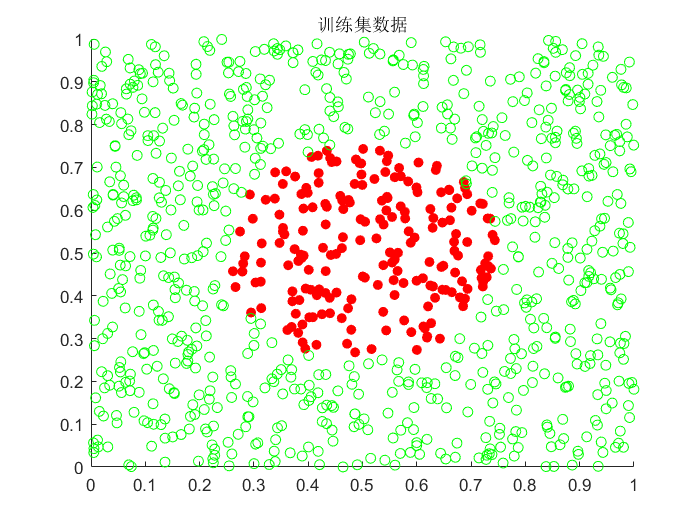
\includegraphics[scale=0.8]{case1/traindata}
  \caption{测试集数据}
  \label{fig:case1:traindata}
\end{figure}

构造数据集的代码如下:

\begin{lstlisting}
%% 构造数据集
data_len = 1000;
data = zeros(data_len,3);
data(:,1:2) = rand(data_len,2);
for i=1:data_len
    data(i,3) = ((data(i,1)-0.5)^2+(data(i,2)-0.5)^2) <= 0.25^2;
end

gindex = find(data(:,3)==0);
rindex = find(data(:,3)==1);

figure;
scatter(data(rindex,1),data(rindex,2),'filled','r');
hold on;
scatter(data(gindex,1),data(gindex,2),'g');
title('训练集数据');
\end{lstlisting}

训练的网络结构使用三层神经元结构,输入层有两个神经元,隐含层有七个神经元,输出层有一个神经元。设置学习步长$step$为$0.5$,期望最高错误率为$1$\%。训练过程的代码如下:

\begin{lstlisting}
%% 训练
levels = [2,7,1];

[W,theta,record] = BP_tranning(data,levels,0.5,3,@compute_error);
\end{lstlisting}

其中$compute\_error$函数如下:

\begin{lstlisting}
function [ error ] = compute_error(output,target)
%COMPUTE_ERROR 此处显示有关此函数的摘要
%   此处显示详细说明
    output(output>0.5)=1;
    output(output<=0.5)=0;
    delta = abs(output - target);
    error = sum(sum(delta))/size(delta,2)*100;
end
\end{lstlisting}

测试神经网络准确性的代码如下:

\begin{lstlisting}
%% 测试
data_len = 1000;
data = zeros(data_len,3);
data(:,1:2) = rand(data_len,2);
for i=1:data_len
    data(i,3) = ((data(i,1)-0.5)^2+(data(i,2)-0.5)^2) <= 0.25^2;
end

Y = predict(data(:,1:2),W,theta);

Y(Y>0.5)=1;
Y(Y<=0.5)=0;
T = data(:,3) - Y';
correct_index = find(T == 0);
green_index = find(data(:,3)==0);
error_index = find(T ~= 0);
red_index = find(data(:,3)==1);

figure;
scatter(data(green_index,1),data(green_index,2),'g');
hold on
scatter(data(red_index,1),data(red_index,2),'filled','r');
title('分类测试结果')
figure;
scatter(data(correct_index,1),data(correct_index,2),'g');
hold on
scatter(data(error_index,1),data(error_index,2),'filled','r');
title('正确点和错误点')
figure;
plot(record);
title('历史错误率');
xlabel('次数');
ylabel('错误率');
\end{lstlisting}

经过分类测试的结果如图~\ref{fig:case1:result}。正确点和错误点图为图~\ref{fig:case1:incorrect},其中,红色实心点代表错误点,绿色空心点代表正确点。历史错误率如图~\ref{fig:case1:record}。

\begin{figure}[h] 
 \centering
  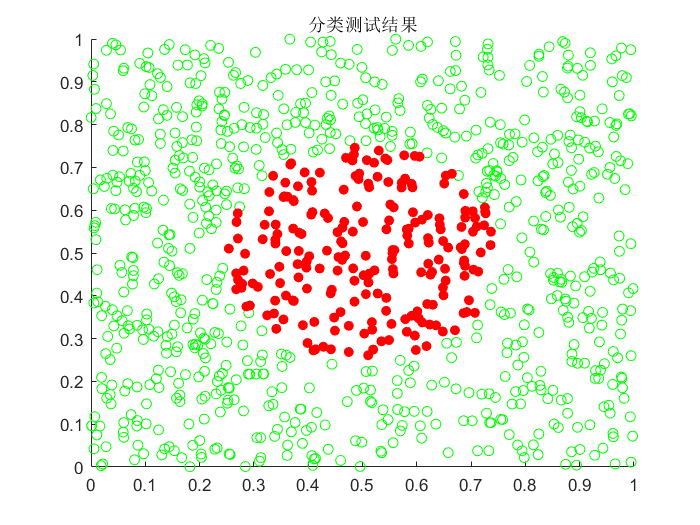
\includegraphics[scale=0.8]{case1/result}
  \caption{分类测试结果}
  \label{fig:case1:result}
\end{figure}
\begin{figure}[h] 
 \centering
  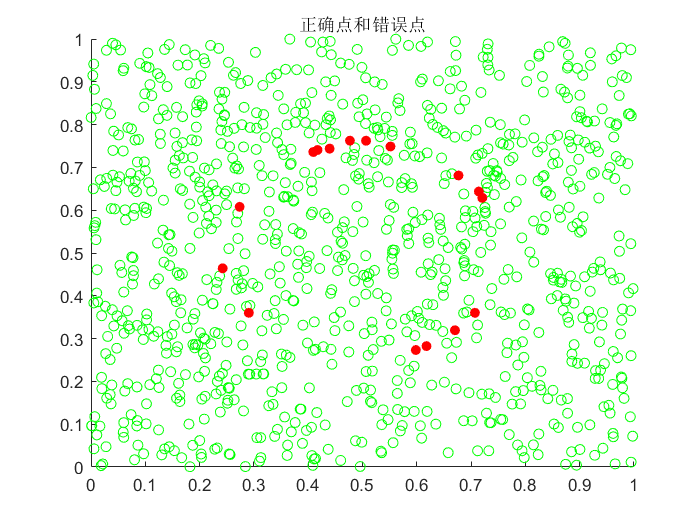
\includegraphics[scale=0.8]{case1/incorrect}
  \caption{正确点和错误点}
  \label{fig:case1:incorrect}
\end{figure}
\begin{figure}[h] 
 \centering
  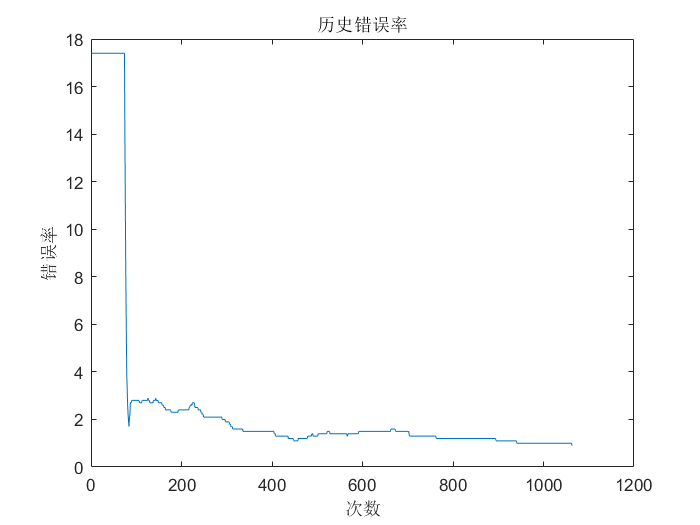
\includegraphics[scale=0.8]{case1/record}
  \caption{历史错误率}
  \label{fig:case1:record}
\end{figure}

现将这个神经网络模型运用到双曲线分类问题中,随机生成的数据集如图~\ref{fig:case2:traindata}

\begin{figure}[h] 
 \centering
  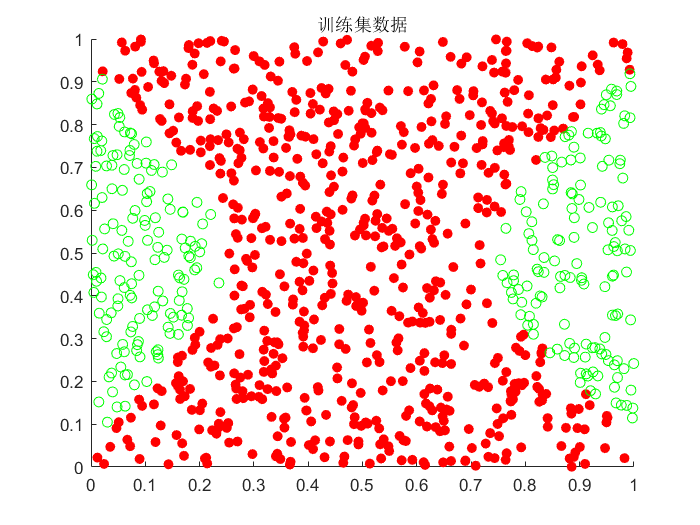
\includegraphics[scale=0.8]{case2/traindata}
  \caption{测试集数据}
  \label{fig:case2:traindata}
\end{figure}

构造数据集的代码如下:

\begin{lstlisting}
%% 构造数据集
data_len = 1000;
data = zeros(data_len,3);
data(:,1:2) = rand(data_len,2);
for i=1:data_len
    data(i,3) = ((data(i,1)-0.5)^2-(data(i,2)-0.5)^2) <= 0.25^2;
end

gindex = find(data(:,3)==0);
rindex = find(data(:,3)==1);

figure;
scatter(data(rindex,1),data(rindex,2),'filled','r');
hold on;
scatter(data(gindex,1),data(gindex,2),'g');
title('训练集数据');
\end{lstlisting}

训练的网络结构使用三层神经元结构,输入层有两个神经元,隐含层有七个神经元,输出层有一个神经元。设置学习步长$step$为$0.5$,期望最高错误率为$1$\%。训练过程的代码如下:

\begin{lstlisting}
%% 训练
levels = [2,7,1];

[W,theta,record] = BP_tranning(data,levels,0.5,3,@compute_error);
\end{lstlisting}

其中$compute\_error$函数如下:

\begin{lstlisting}
function [ error ] = compute_error(output,target)
%COMPUTE_ERROR 此处显示有关此函数的摘要
%   此处显示详细说明
    output(output>0.5)=1;
    output(output<=0.5)=0;
    delta = abs(output - target);
    error = sum(sum(delta))/size(delta,2)*100;
end
\end{lstlisting}

测试神经网络准确性的代码如下:

\begin{lstlisting}
%% 测试
data_len = 1000;
data = zeros(data_len,3);
data(:,1:2) = rand(data_len,2);
for i=1:data_len
    data(i,3) = ((data(i,1)-0.5)^2-(data(i,2)-0.5)^2) <= 0.25^2;
end

Y = predict(data(:,1:2),W,theta);

Y(Y>0.5)=1;
Y(Y<=0.5)=0;
T = data(:,3) - Y';
correct_index = find(T == 0);
green_index = find(data(:,3)==0);
error_index = find(T ~= 0);
red_index = find(data(:,3)==1);

figure;
scatter(data(green_index,1),data(green_index,2),'g');
hold on
scatter(data(red_index,1),data(red_index,2),'filled','r');
title('分类测试结果')
figure;
scatter(data(correct_index,1),data(correct_index,2),'g');
hold on
scatter(data(error_index,1),data(error_index,2),'filled','r');
title('正确点和错误点')
figure;
plot(record);
title('历史错误率');
xlabel('次数');
ylabel('错误率');
\end{lstlisting}

经过分类测试的结果如图~\ref{fig:case2:result}。正确点和错误点图为图~\ref{fig:case2:incorrect},其中,红色实心点代表错误点,绿色空心点代表正确点。历史错误率如图~\ref{fig:case2:record}。

\begin{figure}[h] 
 \centering
  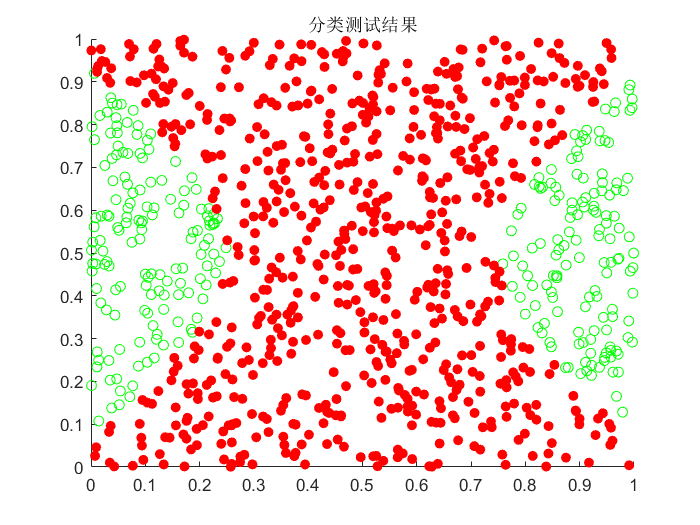
\includegraphics[scale=0.8]{case2/result}
  \caption{分类测试结果}
  \label{fig:case2:result}
\end{figure}
\begin{figure}[h] 
 \centering
  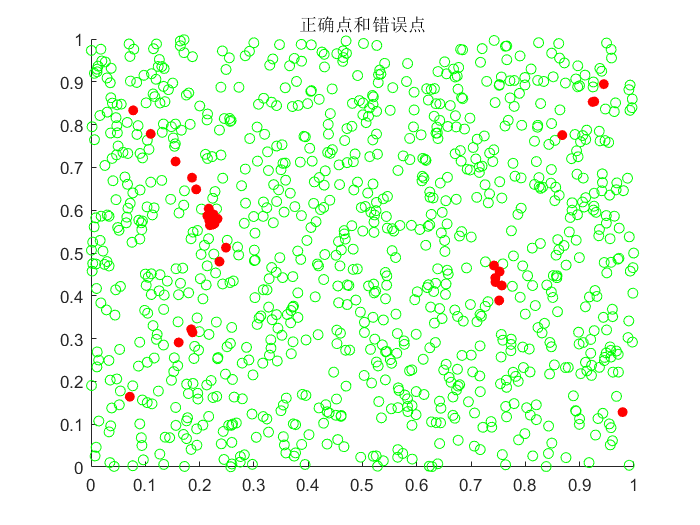
\includegraphics[scale=0.8]{case2/incorrect}
  \caption{正确点和错误点}
  \label{fig:case2:incorrect}
\end{figure}
\begin{figure}[h] 
 \centering
  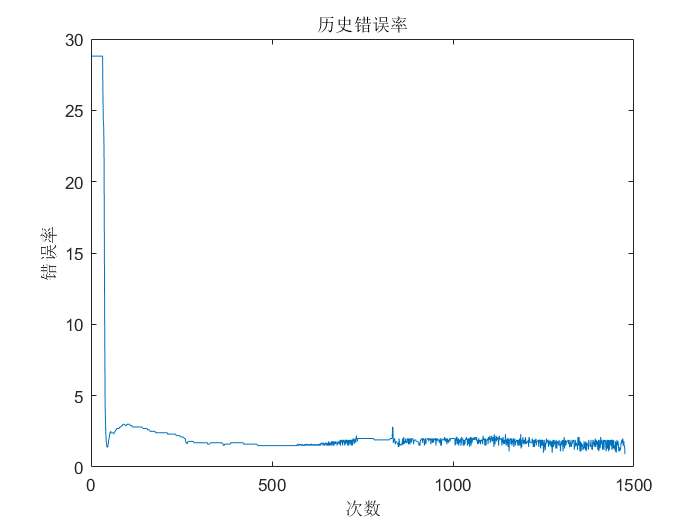
\includegraphics[scale=0.8]{case2/record}
  \caption{历史错误率}
  \label{fig:case2:record}
\end{figure}

\section{三维分类问题}

现将这个神经网络模型运用到三维球形分类问题中,随机生成的数据集如图~\ref{fig:case3:traindata}

\begin{figure}[h] 
 \centering
  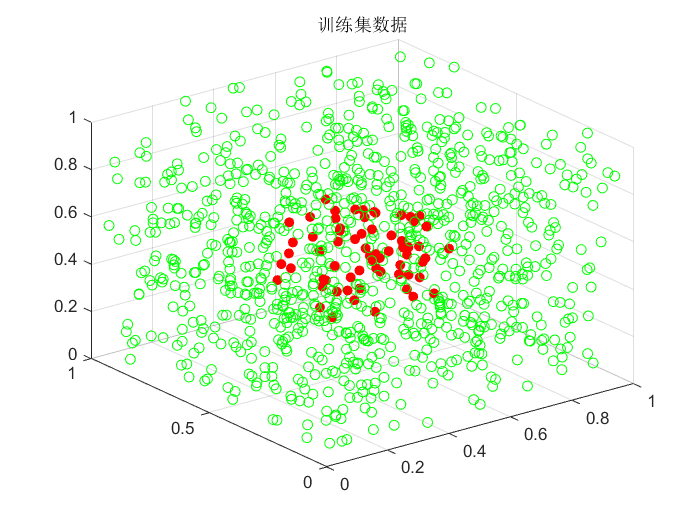
\includegraphics[scale=0.8]{case3/traindata}
  \caption{测试集数据}
  \label{fig:case3:traindata}
\end{figure}

构造数据集的代码如下:

\begin{lstlisting}
%% 构造数据集
data_len = 1000;
data = zeros(data_len,4);
data(:,1:3) = rand(data_len,3);
for i=1:data_len
    data(i,4) = ((data(i,1)-0.5)^2+(data(i,2)-0.5)^2+(data(i,3)-0.5)^2) <= 0.25^2;
end

gindex = find(data(:,4)==0);
rindex = find(data(:,4)==1);

figure;
scatter3(data(rindex,1),data(rindex,2),data(rindex,3),'filled','r');
hold on;
scatter3(data(gindex,1),data(gindex,2),data(gindex,3),'g');
title('训练集数据');
\end{lstlisting}

训练的网络结构使用三层神经元结构,输入层有三个神经元,隐含层有七个神经元,输出层有一个神经元。设置学习步长$step$为$0.5$,期望最高错误率为$1$\%。训练过程的代码如下:

\begin{lstlisting}
%% 训练
levels = [3,7,1];

[W,theta,record] = BP_tranning(data,levels,0.5,1,@compute_error);
\end{lstlisting}

其中$compute\_error$函数如下:

\begin{lstlisting}
function [ error ] = compute_error(output,target)
%COMPUTE_ERROR 此处显示有关此函数的摘要
%   此处显示详细说明
    output(output>0.5)=1;
    output(output<=0.5)=0;
    delta = abs(output - target);
    error = sum(sum(delta))/size(delta,2)*100;
end
\end{lstlisting}

测试神经网络准确性的代码如下:

\begin{lstlisting}
%% 测试
data_len = 1000;
data = zeros(data_len,4);
data(:,1:3) = rand(data_len,3);
for i=1:data_len
    data(i,4) = ((data(i,1)-0.5)^2+(data(i,2)-0.5)^2+(data(i,3)-0.5)^2) <= 0.25^2;
end

Y = predict(data(:,1:3),W,theta);

Y(Y>0.5)=1;
Y(Y<=0.5)=0;
T = data(:,4) - Y';
correct_index = find(T == 0);
green_index = find(data(:,4)==0);
error_index = find(T ~= 0);
red_index = find(data(:,4)==1);

figure;
scatter3(data(green_index,1),data(green_index,2),data(green_index,3),'g');
hold on
scatter3(data(red_index,1),data(red_index,2),data(red_index,3),'filled','r');
title('分类测试结果')
figure;
scatter3(data(correct_index,1),data(correct_index,2),data(correct_index,3),'g');
hold on
scatter3(data(error_index,1),data(error_index,2),data(error_index,3),'filled','r');
title('正确点和错误点')
figure;
plot(record);
title('历史错误率');
xlabel('次数');
ylabel('错误率');
\end{lstlisting}

经过分类测试的结果如图~\ref{fig:case3:result}。正确点和错误点图为图~\ref{fig:case3:incorrect},其中,红色实心点代表错误点,绿色空心点代表正确点。历史错误率如图~\ref{fig:case3:record}。

\begin{figure}[h] 
 \centering
  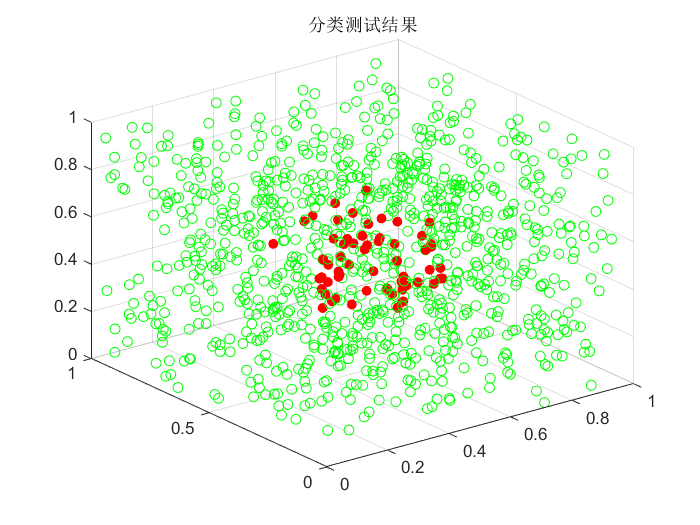
\includegraphics[scale=0.8]{case3/result}
  \caption{分类测试结果}
  \label{fig:case3:result}
\end{figure}
\begin{figure}[h] 
 \centering
  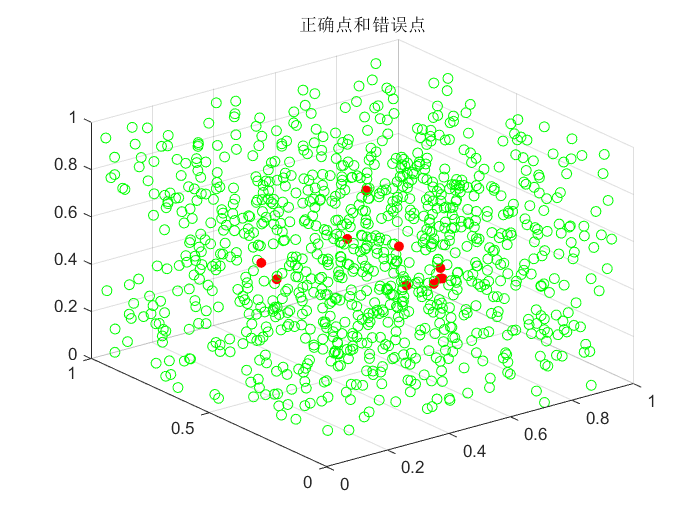
\includegraphics[scale=0.8]{case3/incorrect}
  \caption{正确点和错误点}
  \label{fig:case3:incorrect}
\end{figure}
\begin{figure}[h] 
 \centering
  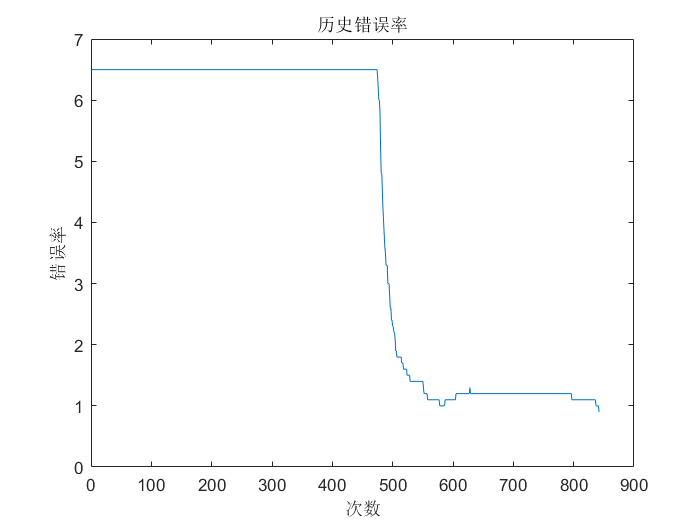
\includegraphics[scale=0.8]{case3/record}
  \caption{历史错误率}
  \label{fig:case3:record}
\end{figure}
\chapter{结论}

本文构建了误差反向传播神经网络的数学模型,并利用Matlab实现了该数学模型,还将此模型运用到二维分类问题和三维分类问题中。采用三层的神经网络模型进行研究,分别为输入层、隐含层和输出层。其中,将点的位置分量作为模型输入层的输入向量,采用$sigmoid$为激活函数。

通过不断地训练,两个问题的正确率均能达到$99\%$以上,且具有良好的性能,但在分类图形的边界上错误率较高。能够较好地解决这类分类问题。在训练过程中,$\eta$的选值比较关键,在训练后期,错误率容易上下波动,难以收敛。

误差反向传播神经网络摆脱了传统方式的局限,突破了依赖线性模型的限制,但在训练后期,常出现错误率不稳定等问题,本文所构建的模型未能在函数逼近拟合等问题上得到很好的应用,因此,在后续研究中模型仍需改进。



%%% 其它部分
\backmatter

%% 本科生要这几个索引,研究生不要。选择性留下。
% 插图索引
\listoffigures
% 表格索引
% \listoftables
% 公式索引
\listofequations


%% 参考文献
% 注意:至少需要引用一篇参考文献,否则下面两行可能引起编译错误。
% 如果不需要参考文献,请将下面两行删除或注释掉。
% 数字式引用
\bibliographystyle{thuthesis-numeric}
% 作者-年份式引用
% \bibliographystyle{thuthesis-author-year}
\bibliography{ref/refs}


%% 致谢
% % 如果使用声明扫描页,将可选参数指定为扫描后的 PDF 文件名,例如:
% \begin{acknowledgement}[scan-statement.pdf]
\begin{acknowledgement}
  衷心感谢导师 xxx 教授和物理系 xxx 副教授对本人的精心指导。他们的言传身教将使
  我终生受益。

  在美国麻省理工学院化学系进行九个月的合作研究期间,承蒙 xxx 教授热心指导与帮助,不
  胜感激。感谢 xx 实验室主任 xx 教授,以及实验室全体老师和同学们的热情帮助和支
  持!本课题承蒙国家自然科学基金资助,特此致谢。

  感谢 \LaTeX 和 \thuthesis\cite{thuthesis},帮我节省了不少时间。
\end{acknowledgement}


%% 附录
% \begin{appendix}
% \chapter{外文资料原文}
\label{cha:engorg}

\title{The title of the English paper}

\textbf{Abstract:} As one of the most widely used techniques in operations
research, \emph{ mathematical programming} is defined as a means of maximizing a
quantity known as \emph{bjective function}, subject to a set of constraints
represented by equations and inequalities. Some known subtopics of mathematical
programming are linear programming, nonlinear programming, multiobjective
programming, goal programming, dynamic programming, and multilevel
programming$^{[1]}$.

It is impossible to cover in a single chapter every concept of mathematical
programming. This chapter introduces only the basic concepts and techniques of
mathematical programming such that readers gain an understanding of them
throughout the book$^{[2,3]}$.


\section{Single-Objective Programming}
The general form of single-objective programming (SOP) is written
as follows,
\begin{equation}\tag*{(123)} % 如果附录中的公式不想让它出现在公式索引中,那就请
                             % 用 \tag*{xxxx}
\left\{\begin{array}{l}
\max \,\,f(x)\\[0.1 cm]
\mbox{subject to:} \\ [0.1 cm]
\qquad g_j(x)\le 0,\quad j=1,2,\cdots,p
\end{array}\right.
\end{equation}
which maximizes a real-valued function $f$ of
$x=(x_1,x_2,\cdots,x_n)$ subject to a set of constraints.

\newtheorem{mpdef}{Definition}[chapter]
\begin{mpdef}
In SOP, we call $x$ a decision vector, and
$x_1,x_2,\cdots,x_n$ decision variables. The function
$f$ is called the objective function. The set
\begin{equation}\tag*{(456)} % 这里同理,其它不再一一指定。
S=\left\{x\in\Re^n\bigm|g_j(x)\le 0,\,j=1,2,\cdots,p\right\}
\end{equation}
is called the feasible set. An element $x$ in $S$ is called a
feasible solution.
\end{mpdef}

\newtheorem{mpdefop}[mpdef]{Definition}
\begin{mpdefop}
A feasible solution $x^*$ is called the optimal
solution of SOP if and only if
\begin{equation}
f(x^*)\ge f(x)
\end{equation}
for any feasible solution $x$.
\end{mpdefop}

One of the outstanding contributions to mathematical programming was known as
the Kuhn-Tucker conditions\ref{eq:ktc}. In order to introduce them, let us give
some definitions. An inequality constraint $g_j(x)\le 0$ is said to be active at
a point $x^*$ if $g_j(x^*)=0$. A point $x^*$ satisfying $g_j(x^*)\le 0$ is said
to be regular if the gradient vectors $\nabla g_j(x)$ of all active constraints
are linearly independent.

Let $x^*$ be a regular point of the constraints of SOP and assume that all the
functions $f(x)$ and $g_j(x),j=1,2,\cdots,p$ are differentiable. If $x^*$ is a
local optimal solution, then there exist Lagrange multipliers
$\lambda_j,j=1,2,\cdots,p$ such that the following Kuhn-Tucker conditions hold,
\begin{equation}
\label{eq:ktc}
\left\{\begin{array}{l}
    \nabla f(x^*)-\sum\limits_{j=1}^p\lambda_j\nabla g_j(x^*)=0\\[0.3cm]
    \lambda_jg_j(x^*)=0,\quad j=1,2,\cdots,p\\[0.2cm]
    \lambda_j\ge 0,\quad j=1,2,\cdots,p.
\end{array}\right.
\end{equation}
If all the functions $f(x)$ and $g_j(x),j=1,2,\cdots,p$ are convex and
differentiable, and the point $x^*$ satisfies the Kuhn-Tucker conditions
(\ref{eq:ktc}), then it has been proved that the point $x^*$ is a global optimal
solution of SOP.

\subsection{Linear Programming}
\label{sec:lp}

If the functions $f(x),g_j(x),j=1,2,\cdots,p$ are all linear, then SOP is called
a {\em linear programming}.

The feasible set of linear is always convex. A point $x$ is called an extreme
point of convex set $S$ if $x\in S$ and $x$ cannot be expressed as a convex
combination of two points in $S$. It has been shown that the optimal solution to
linear programming corresponds to an extreme point of its feasible set provided
that the feasible set $S$ is bounded. This fact is the basis of the {\em simplex
  algorithm} which was developed by Dantzig as a very efficient method for
solving linear programming.
\begin{table}[ht]
\centering
  \centering
  \caption*{Table~1\hskip1em This is an example for manually numbered table, which
    would not appear in the list of tables}
  \label{tab:badtabular2}
  \begin{tabular}[c]{|m{1.5cm}|c|c|c|c|c|c|}\hline
    \multicolumn{2}{|c|}{Network Topology} & \# of nodes &
    \multicolumn{3}{c|}{\# of clients} & Server \\\hline
    GT-ITM & Waxman Transit-Stub & 600 &
    \multirow{2}{2em}{2\%}&
    \multirow{2}{2em}{10\%}&
    \multirow{2}{2em}{50\%}&
    \multirow{2}{1.2in}{Max. Connectivity}\\\cline{1-3}
    \multicolumn{2}{|c|}{Inet-2.1} & 6000 & & & &\\\hline
    \multirow{2}{1.5cm}{Xue} & Rui  & Ni &\multicolumn{4}{c|}{\multirow{2}*{\thuthesis}}\\\cline{2-3}
    & \multicolumn{2}{c|}{ABCDEF} &\multicolumn{4}{c|}{} \\\hline
\end{tabular}
\end{table}

Roughly speaking, the simplex algorithm examines only the extreme points of the
feasible set, rather than all feasible points. At first, the simplex algorithm
selects an extreme point as the initial point. The successive extreme point is
selected so as to improve the objective function value. The procedure is
repeated until no improvement in objective function value can be made. The last
extreme point is the optimal solution.

\subsection{Nonlinear Programming}

If at least one of the functions $f(x),g_j(x),j=1,2,\cdots,p$ is nonlinear, then
SOP is called a {\em nonlinear programming}.

A large number of classical optimization methods have been developed to treat
special-structural nonlinear programming based on the mathematical theory
concerned with analyzing the structure of problems.
\begin{figure}[h]
  \centering
  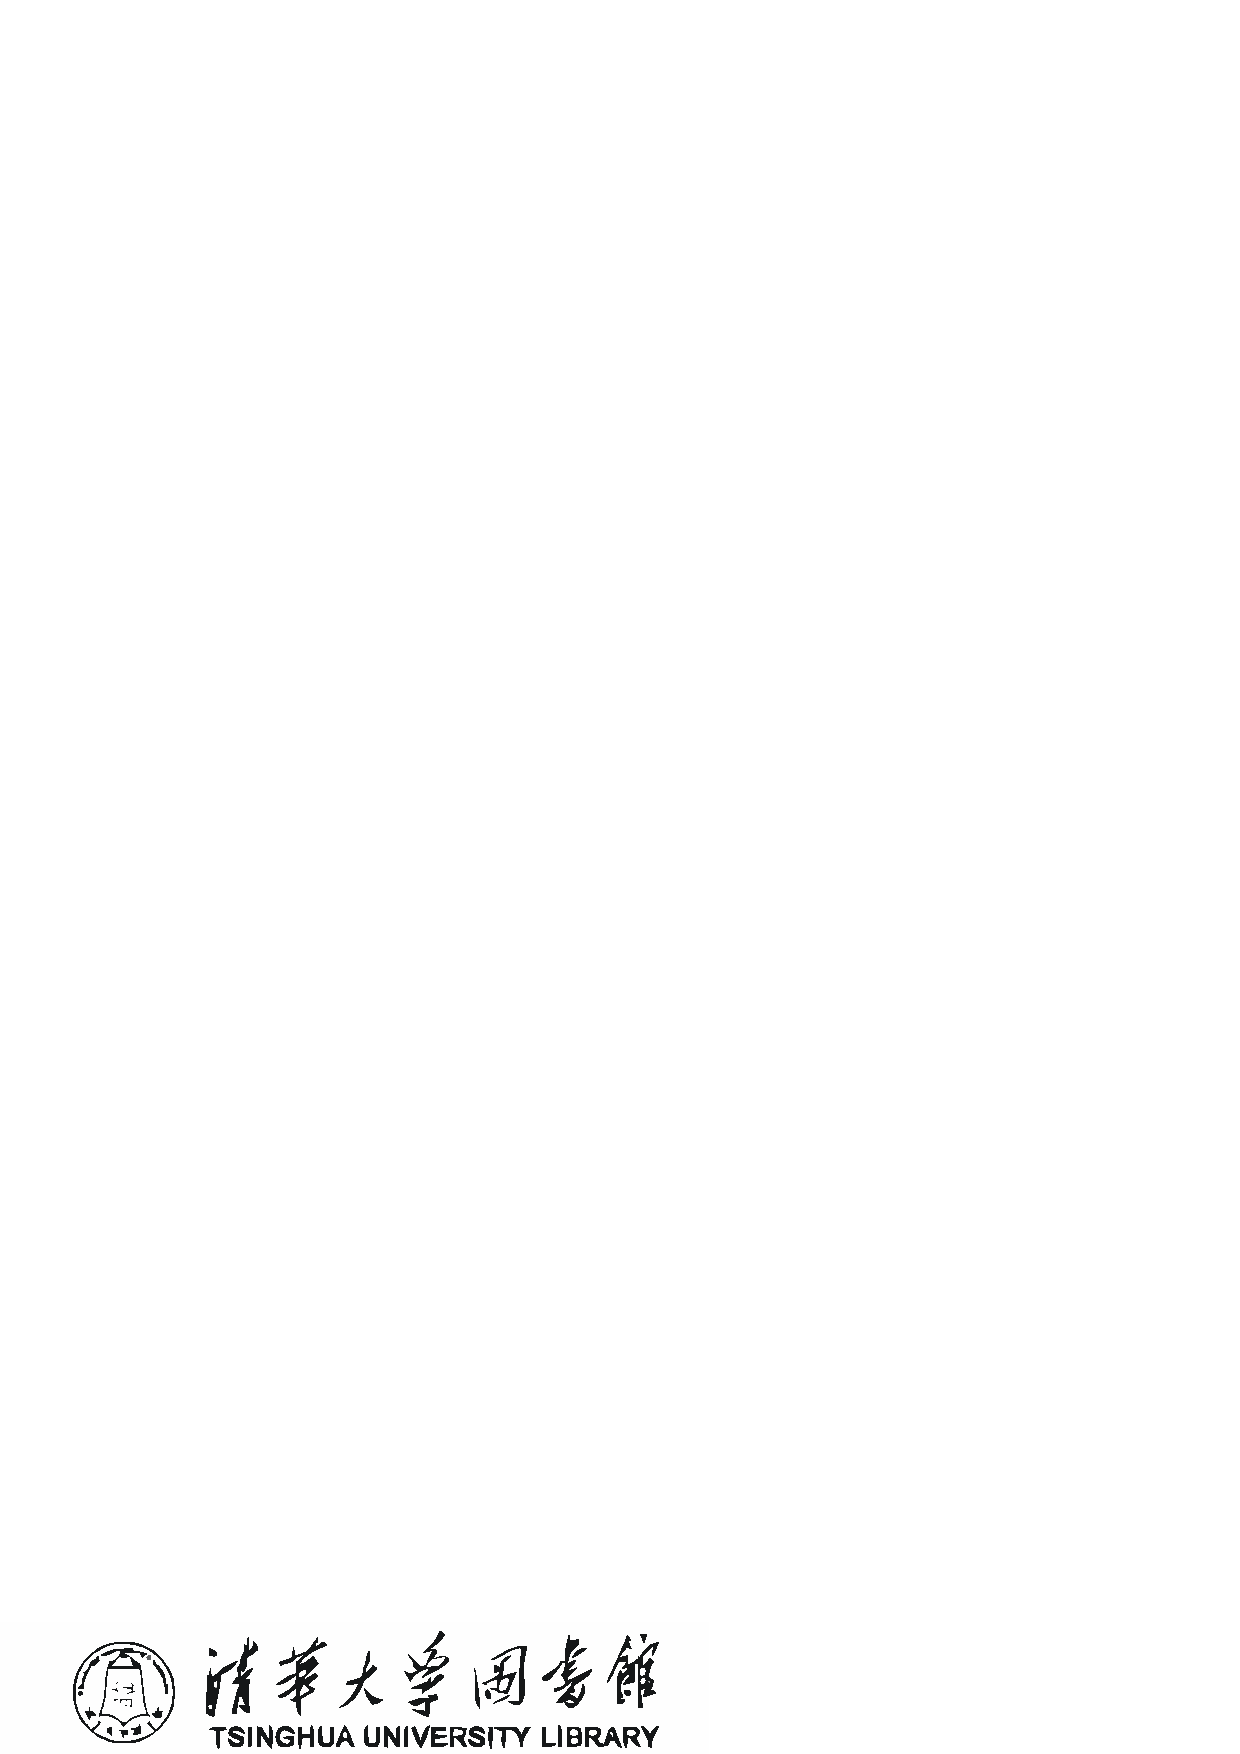
\includegraphics{thu-lib-logo}
  \caption*{Figure~1\quad This is an example for manually numbered figure,
    which would not appear in the list of figures}
  \label{tab:badfigure2}
\end{figure}

Now we consider a nonlinear programming which is confronted solely with
maximizing a real-valued function with domain $\Re^n$.  Whether derivatives are
available or not, the usual strategy is first to select a point in $\Re^n$ which
is thought to be the most likely place where the maximum exists. If there is no
information available on which to base such a selection, a point is chosen at
random. From this first point an attempt is made to construct a sequence of
points, each of which yields an improved objective function value over its
predecessor. The next point to be added to the sequence is chosen by analyzing
the behavior of the function at the previous points. This construction continues
until some termination criterion is met. Methods based upon this strategy are
called {\em ascent methods}, which can be classified as {\em direct methods},
{\em gradient methods}, and {\em Hessian methods} according to the information
about the behavior of objective function $f$. Direct methods require only that
the function can be evaluated at each point. Gradient methods require the
evaluation of first derivatives of $f$. Hessian methods require the evaluation
of second derivatives. In fact, there is no superior method for all
problems. The efficiency of a method is very much dependent upon the objective
function.

\subsection{Integer Programming}

{\em Integer programming} is a special mathematical programming in which all of
the variables are assumed to be only integer values. When there are not only
integer variables but also conventional continuous variables, we call it {\em
  mixed integer programming}. If all the variables are assumed either 0 or 1,
then the problem is termed a {\em zero-one programming}. Although integer
programming can be solved by an {\em exhaustive enumeration} theoretically, it
is impractical to solve realistically sized integer programming problems. The
most successful algorithm so far found to solve integer programming is called
the {\em branch-and-bound enumeration} developed by Balas (1965) and Dakin
(1965). The other technique to integer programming is the {\em cutting plane
  method} developed by Gomory (1959).

\hfill\textit{Uncertain Programming\/}\quad(\textsl{BaoDing Liu, 2006.2})

\section*{References}
\noindent{\itshape NOTE: These references are only for demonstration. They are
  not real citations in the original text.}

\begin{translationbib}
\item Donald E. Knuth. The \TeX book. Addison-Wesley, 1984. ISBN: 0-201-13448-9
\item Paul W. Abrahams, Karl Berry and Kathryn A. Hargreaves. \TeX\ for the
  Impatient. Addison-Wesley, 1990. ISBN: 0-201-51375-7
\item David Salomon. The advanced \TeX book.  New York : Springer, 1995. ISBN:0-387-94556-3
\end{translationbib}

\chapter{外文资料的调研阅读报告或书面翻译}

\title{英文资料的中文标题}

{\heiti 摘要:} 本章为外文资料翻译内容。如果有摘要可以直接写上来,这部分好像没有
明确的规定。

\section{单目标规划}
北冥有鱼,其名为鲲。鲲之大,不知其几千里也。化而为鸟,其名为鹏。鹏之背,不知其几
千里也。怒而飞,其翼若垂天之云。是鸟也,海运则将徙于南冥。南冥者,天池也。
\begin{equation}\tag*{(123)}
 p(y|\mathbf{x}) = \frac{p(\mathbf{x},y)}{p(\mathbf{x})}=
\frac{p(\mathbf{x}|y)p(y)}{p(\mathbf{x})}
\end{equation}

吾生也有涯,而知也无涯。以有涯随无涯,殆已!已而为知者,殆而已矣!为善无近名,为
恶无近刑,缘督以为经,可以保身,可以全生,可以养亲,可以尽年。

\subsection{线性规划}
庖丁为文惠君解牛,手之所触,肩之所倚,足之所履,膝之所倚,砉然响然,奏刀騞然,莫
不中音,合于桑林之舞,乃中经首之会。
\begin{table}[ht]
\centering
  \centering
  \caption*{表~1\hskip1em 这是手动编号但不出现在索引中的一个表格例子}
  \label{tab:badtabular3}
  \begin{tabular}[c]{|m{1.5cm}|c|c|c|c|c|c|}\hline
    \multicolumn{2}{|c|}{Network Topology} & \# of nodes &
    \multicolumn{3}{c|}{\# of clients} & Server \\\hline
    GT-ITM & Waxman Transit-Stub & 600 &
    \multirow{2}{2em}{2\%}&
    \multirow{2}{2em}{10\%}&
    \multirow{2}{2em}{50\%}&
    \multirow{2}{1.2in}{Max. Connectivity}\\\cline{1-3}
    \multicolumn{2}{|c|}{Inet-2.1} & 6000 & & & &\\\hline
    \multirow{2}{1.5cm}{Xue} & Rui  & Ni &\multicolumn{4}{c|}{\multirow{2}*{\thuthesis}}\\\cline{2-3}
    & \multicolumn{2}{c|}{ABCDEF} &\multicolumn{4}{c|}{} \\\hline
\end{tabular}
\end{table}

文惠君曰:“嘻,善哉!技盖至此乎?”庖丁释刀对曰:“臣之所好者道也,进乎技矣。始臣之
解牛之时,所见无非全牛者;三年之后,未尝见全牛也;方今之时,臣以神遇而不以目视,
官知止而神欲行。依乎天理,批大郤,导大窾,因其固然。技经肯綮之未尝,而况大坬乎!
良庖岁更刀,割也;族庖月更刀,折也;今臣之刀十九年矣,所解数千牛矣,而刀刃若新发
于硎。彼节者有间而刀刃者无厚,以无厚入有间,恢恢乎其于游刃必有余地矣。是以十九年
而刀刃若新发于硎。虽然,每至于族,吾见其难为,怵然为戒,视为止,行为迟,动刀甚微,
謋然已解,如土委地。提刀而立,为之而四顾,为之踌躇满志,善刀而藏之。”

文惠君曰:“善哉!吾闻庖丁之言,得养生焉。”


\subsection{非线性规划}
孔子与柳下季为友,柳下季之弟名曰盗跖。盗跖从卒九千人,横行天下,侵暴诸侯。穴室枢
户,驱人牛马,取人妇女。贪得忘亲,不顾父母兄弟,不祭先祖。所过之邑,大国守城,小
国入保,万民苦之。孔子谓柳下季曰:“夫为人父者,必能诏其子;为人兄者,必能教其弟。
若父不能诏其子,兄不能教其弟,则无贵父子兄弟之亲矣。今先生,世之才士也,弟为盗
跖,为天下害,而弗能教也,丘窃为先生羞之。丘请为先生往说之。”
\begin{figure}[h]
  \centering
  
\includegraphics{thu-whole-logo}
  \caption*{图~1\hskip1em 这是手动编号但不出现索引中的图片的例子}
  \label{tab:badfigure3}
\end{figure}

柳下季曰:“先生言为人父者必能诏其子,为人兄者必能教其弟,若子不听父之诏,弟不受
兄之教,虽今先生之辩,将奈之何哉?且跖之为人也,心如涌泉,意如飘风,强足以距敌,
辩足以饰非。顺其心则喜,逆其心则怒,易辱人以言。先生必无往。”

孔子不听,颜回为驭,子贡为右,往见盗跖。

\subsection{整数规划}
盗跖乃方休卒徒大山之阳,脍人肝而餔之。孔子下车而前,见谒者曰:“鲁人孔丘,闻将军
高义,敬再拜谒者。”谒者入通。盗跖闻之大怒,目如明星,发上指冠,曰:“此夫鲁国之
巧伪人孔丘非邪?为我告之:尔作言造语,妄称文、武,冠枝木之冠,带死牛之胁,多辞缪
说,不耕而食,不织而衣,摇唇鼓舌,擅生是非,以迷天下之主,使天下学士不反其本,妄
作孝弟,而侥幸于封侯富贵者也。子之罪大极重,疾走归!不然,我将以子肝益昼餔之膳。”


\chapter{其它附录}
前面两个附录主要是给本科生做例子。其它附录的内容可以放到这里,当然如果你愿意,可
以把这部分也放到独立的文件中,然后将其 \cs{input} 到主文件中。

% \end{appendix}

%% 个人简历
%  \begin{resume}

  \resumeitem{个人简历}

  xxxx 年 xx 月 xx 日出生于 xx 省 xx 县。

  xxxx 年 9 月考入 xx 大学 xx 系 xx 专业,xxxx 年 7 月本科毕业并获得 xx 学士学位。

  xxxx 年 9 月免试进入 xx 大学 xx 系攻读 xx 学位至今。

  \researchitem{发表的学术论文} % 发表的和录用的合在一起

  % 1. 已经刊载的学术论文(本人是第一作者,或者导师为第一作者本人是第二作者)
  \begin{publications}
    \item Yang Y, Ren T L, Zhang L T, et al. Miniature microphone with silicon-
      based ferroelectric thin films. Integrated Ferroelectrics, 2003,
      52:229-235. (SCI 收录, 检索号:758FZ.)
    \item 杨轶, 张宁欣, 任天令, 等. 硅基铁电微声学器件中薄膜残余应力的研究. 中国机
      械工程, 2005, 16(14):1289-1291. (EI 收录, 检索号:0534931 2907.)
    \item 杨轶, 张宁欣, 任天令, 等. 集成铁电器件中的关键工艺研究. 仪器仪表学报,
      2003, 24(S4):192-193. (EI 源刊.)
  \end{publications}

  % 2. 尚未刊载,但已经接到正式录用函的学术论文(本人为第一作者,或者
  %    导师为第一作者本人是第二作者)。
  \begin{publications}[before=\publicationskip,after=\publicationskip]
    \item Yang Y, Ren T L, Zhu Y P, et al. PMUTs for handwriting recognition. In
      press. (已被 Integrated Ferroelectrics 录用. SCI 源刊.)
  \end{publications}

  % 3. 其他学术论文。可列出除上述两种情况以外的其他学术论文,但必须是
  %    已经刊载或者收到正式录用函的论文。
  \begin{publications}
    \item Wu X M, Yang Y, Cai J, et al. Measurements of ferroelectric MEMS
      microphones. Integrated Ferroelectrics, 2005, 69:417-429. (SCI 收录, 检索号
      :896KM)
    \item 贾泽, 杨轶, 陈兢, 等. 用于压电和电容微麦克风的体硅腐蚀相关研究. 压电与声
      光, 2006, 28(1):117-119. (EI 收录, 检索号:06129773469)
    \item 伍晓明, 杨轶, 张宁欣, 等. 基于MEMS技术的集成铁电硅微麦克风. 中国集成电路,
      2003, 53:59-61.
  \end{publications}

  \researchitem{研究成果} % 有就写,没有就删除
  \begin{achievements}
    \item 任天令, 杨轶, 朱一平, 等. 硅基铁电微声学传感器畴极化区域控制和电极连接的
      方法: 中国, CN1602118A. (中国专利公开号)
    \item Ren T L, Yang Y, Zhu Y P, et al. Piezoelectric micro acoustic sensor
      based on ferroelectric materials: USA, No.11/215, 102. (美国发明专利申请号)
  \end{achievements}

\end{resume}


%% 本科生进行格式审查是需要下面这个表格,答辩可能不需要。选择性留下。
% 综合论文训练记录表
% 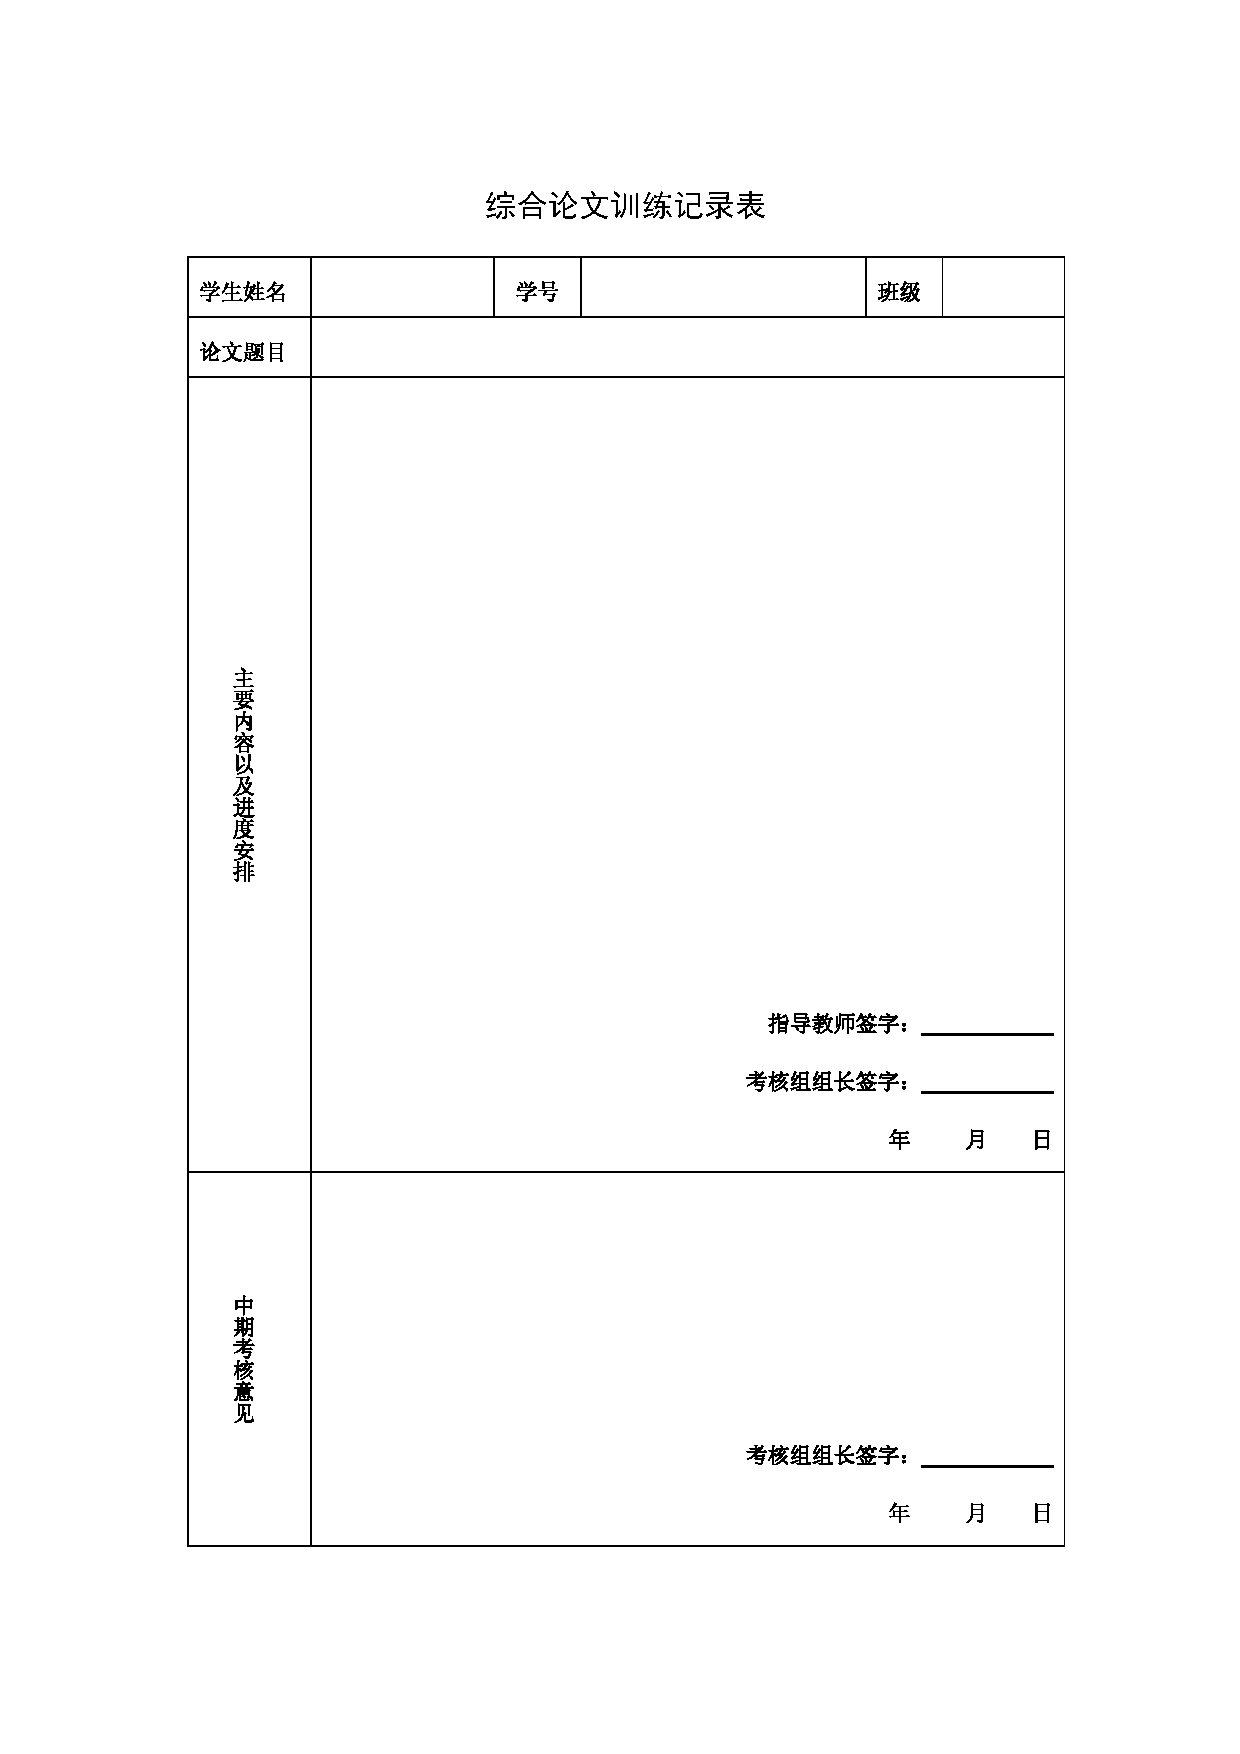
\includepdf[pages=-]{scan-record.pdf}
\end{document}
